\chapter{文字与图表}
\section{文字}
每章的标题以\textbf{三号黑体字}居中打印;“章”下\cemph{空两行}为节的标题,以\textbf{四号黑体字}左起打印;“节”下空一行为小节的标题,以\textbf{小四号黑体字}左起打印。换行后打印论文正文。文字的行间距20磅,字符为标准间距。

\subsection{数值与单位}

单位采用宏包\href{http://mirrors.sjtug.sjtu.edu.cn/ctan/macros/latex/contrib/siunitx/siunitx.pdf}{\textit{siunitx}}插入,例如传输速率是$\SI{100}{\mega\byte}$,信噪比为$\SI{20}{\mdecibel}$。(注意,如果要使用字节单位,则需要增加选项\cemph{binary-units}) 

引用一个表格\ref{chap:notation}。

\section{表}

\begin{table*}[!htb]
	\centering
	\caption{数学符号含义表(标题及序号置于表的正上方)}
	\label{chap:notation}
	\begin{tabular}{|c|c||c|c|}
		\hline
		\rowcolor{LightSteelBlue}
		\textbf{符号} 			& \textbf{含义} 	    & \textbf{符号}		  & \textbf{含义} 		   	 \\
		\hline
		$N$ 					 & 数量		   		 & $\mathbb{N}$ 		 & 集合 						\\
		\hline
		$\gamma$ 				 & 信噪比			    & $\mathcal{T}$ 		& 时刻		 			   \\
		\hline
	\end{tabular}
\end{table*}

\section{图}

\begin{figure}
	\centering
	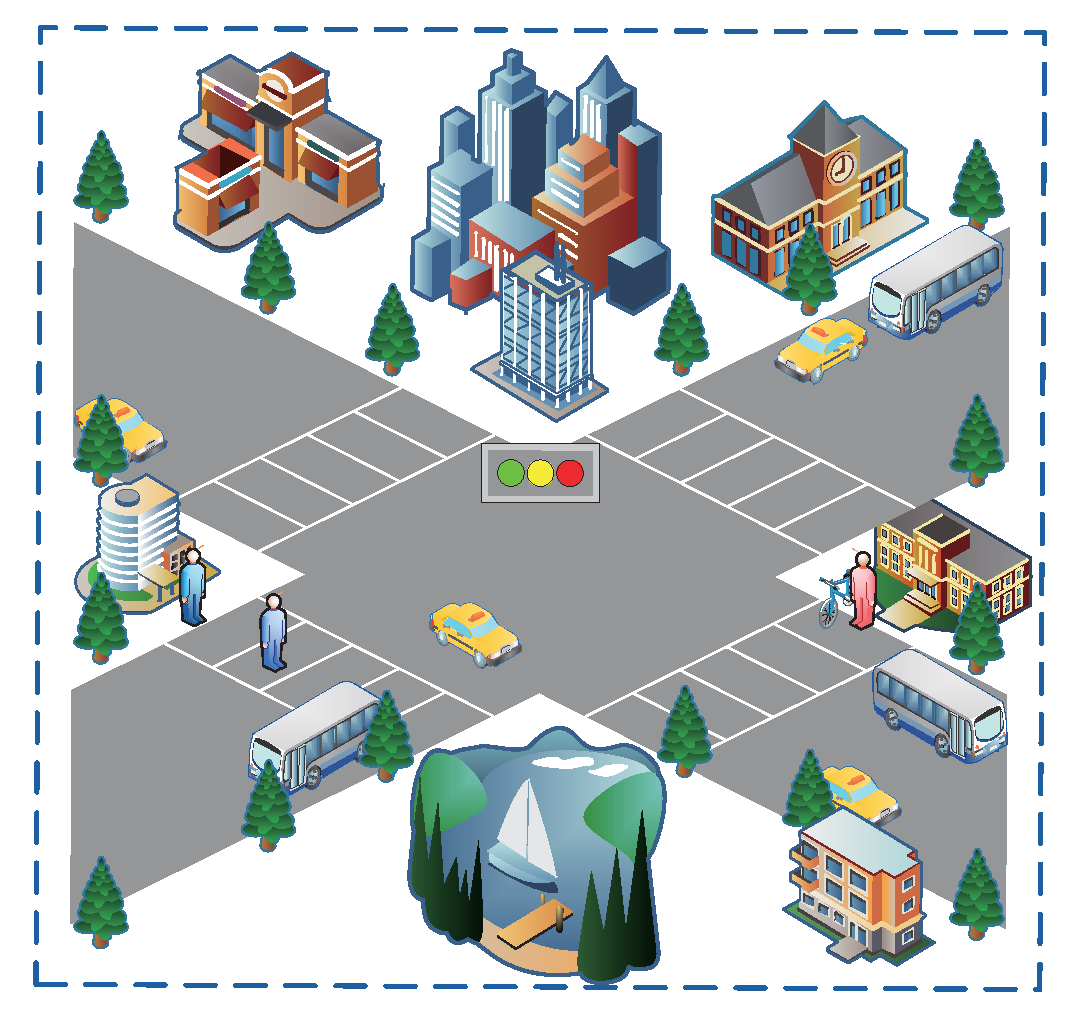
\includegraphics[width=0.8\textwidth]{scenario.eps}
	\caption{场景示意图(五号楷体)}
	\label{chap:scenario}
\end{figure}

图\ref{chap:scenario}展示了xxx。

\begin{figure}[!htb]
	\centering
	\begin{minipage}{0.48\textwidth}
		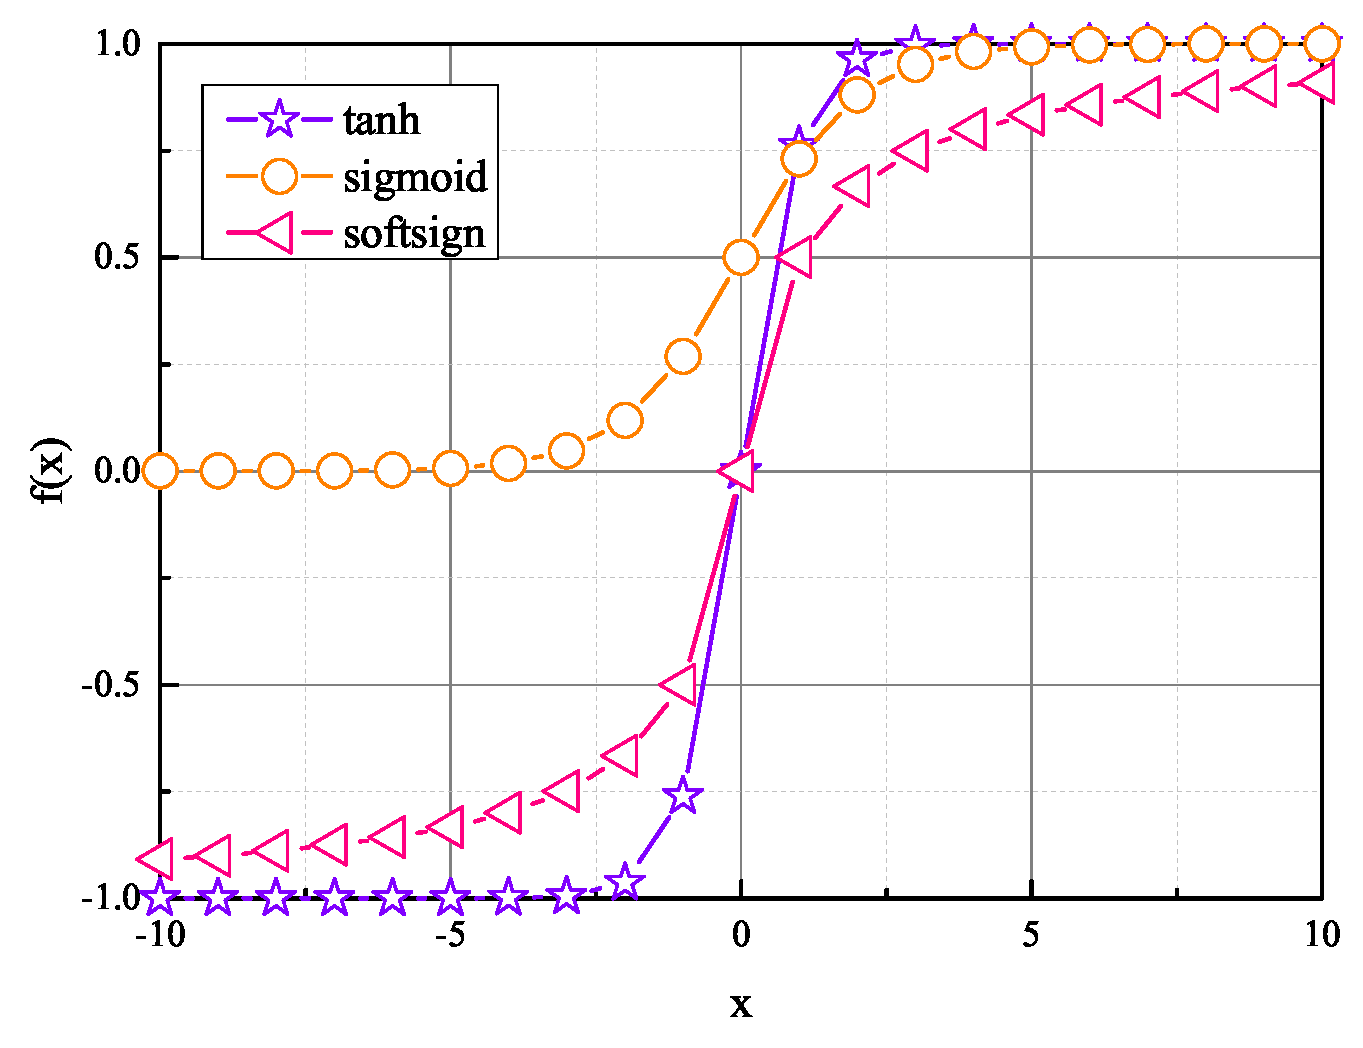
\includegraphics[width=\textwidth]{activation.eps}
		\caption{激活函数}
		\label{chap:activation}
	\end{minipage}
	\begin{minipage}{0.48\textwidth}
		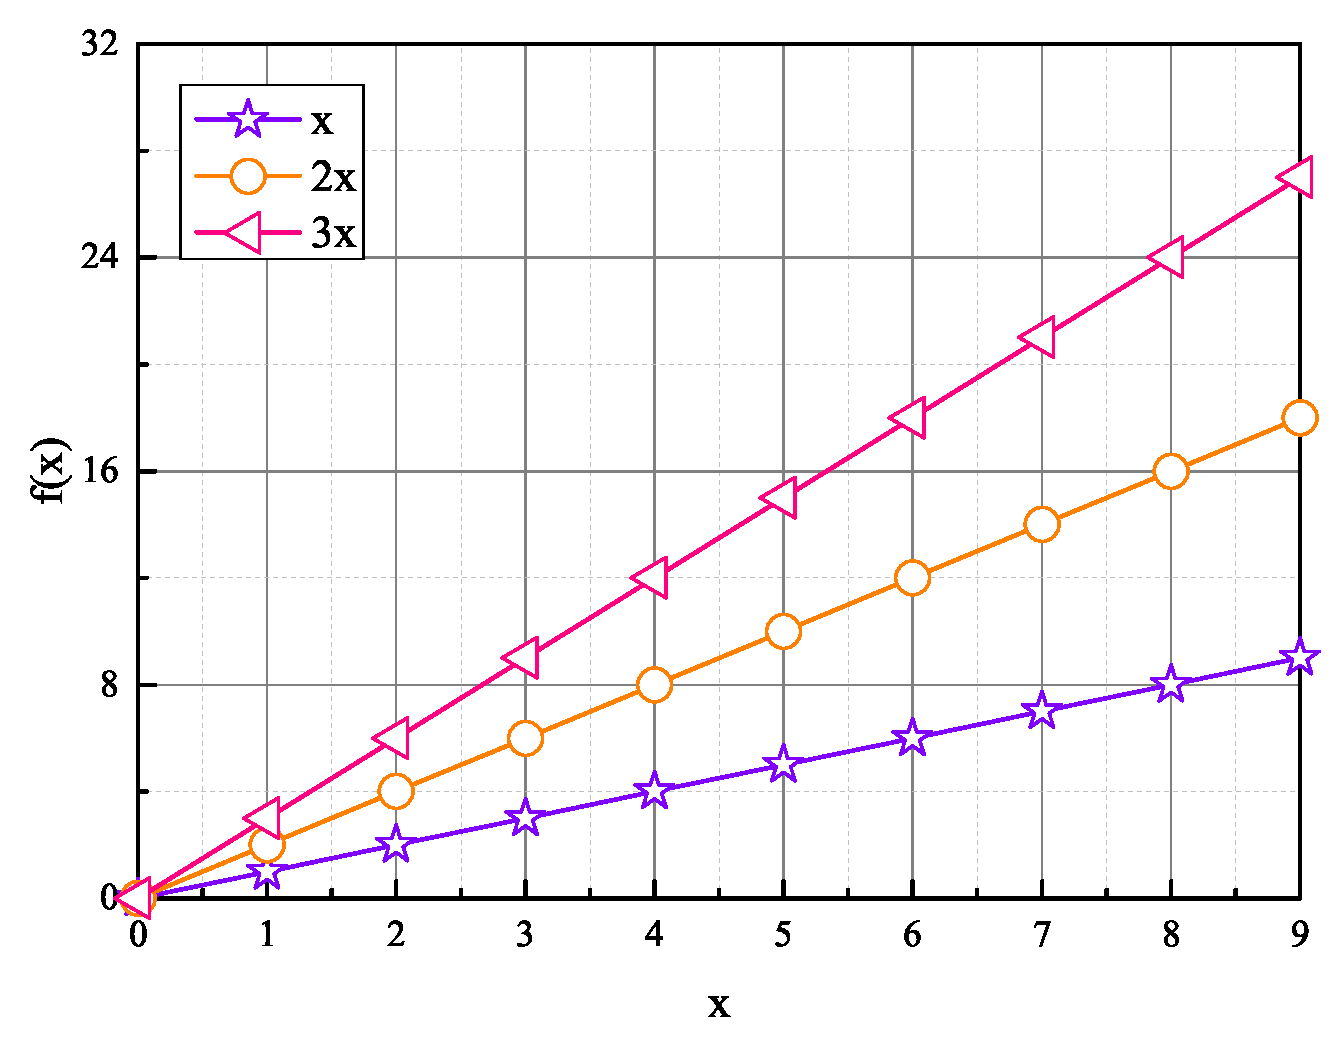
\includegraphics[width=\textwidth]{linear.eps}
		\caption{线性函数}
		\label{chap:linear}
	\end{minipage}
\end{figure}

激活函数\ref{chap:activation},线性函数\ref{chap:linear}

